\documentclass[12pt,letterpaper]{article}

\usepackage[T1]{fontenc}
\usepackage[margin=1in,headheight=1.5em]{geometry}
\usepackage{enumerate}
\usepackage{fancyhdr}
\usepackage{lastpage}
\usepackage{float}
\usepackage{tabu}
\usepackage{booktabs}
\usepackage{graphicx}
\usepackage{lmodern}

\begin{document}

\renewcommand\headrule{}

\pagestyle{fancy}
\fancyhf{}
\lfoot{COMP 3004}
\rfoot{\thepage/\pageref{LastPage}}
\cfoot{Requirements Analysis Document}

\newcommand{\personone}{Kevin Hua}
\newcommand{\persontwo}{Henri Knoetze}
\newcommand{\personthree}{Juhandr\'e Knoetze}
\thispagestyle{empty}

\begin{center}
CARLETON UNIVERSITY
\end{center}

\vfill

\begin{center}
{\fontsize{55pt}{55pt}\selectfont cuPID}
\vspace{0.5em}\rule{\textwidth}{0.5pt}
Requirements Analysis Document
\end{center}

\vspace{5em}

\begin{center}
\textbf{Team [Code First, Think Later]}\\
\personone{}\\
\persontwo{}\\
\personthree{}
\end{center}

\vfill

\begin{center}
Submitted to:\\
Dr. Christine Laurendeau\\
COMP 3004: Object Oriented Software Engineering\\
School of Computer Science\\
Carleton University
\end{center}

\vspace{2em}

\begin{center}
\today
\end{center}

\newpage{}

\tableofcontents{}

\renewcommand{\listfigurename}{Figures}
\listoffigures

\renewcommand{\listtablename}{Tables}
\listoftables

\newpage{}

\section{Introduction}

\begin{center}
-- project --
\end{center}

\begin{center}
{\Huge [cuPID]}
\end{center}

\begin{center}
\rule{0.85\textwidth}{0.5pt}
\end{center}

\subsection{Purpose of System}

Team projects are typically assigned in University courses in order to develop and foster
good teamwork related skills, which are crucial in most future endeavours, notably 
prospective employment. Unfortunately, the task of separating students into balanced 
and compatible teams has always been a nigh impossible feat - hardly a year passes that doesn't
boast at least a single team brimming with  contention. There just seems to be too many
nuances that are involved in building a perfect team for professors to account for, often leading
to random or pseudo-random assignment of teams. Another possibility that professors might employ
would be to allow the students themselves to form their teams. Regrettably, this option also
leads to much strife - students tend to select friends or acquaintances as partners. While this
solution might seem good, it is sadly the case that good friends often make bad project partners. 
There is also the case that many students have not made friends or acquaintances yet that they 
could ask to be their partners, thus leaving them to form a team with others in their situation.

Both current options leave much to be desired. Our firm, [Code First, Think Later], has been hired
to design a system that would provide a better solution to this long-standing issue. Thus, the purpose of
our system is to separate students into teams with others of similar personality and skills, eliminating 
the frequent torment associated with ill-matched teams.

\subsection{Overview of Document}



\vspace{1em}

\noindent Best regards,

\vspace{1em}

\textbf{Team [Code First, Think Later]}

\newpage{}

\section{Proposed System}

\subsection{Overview}


\subsection{Functional Requirements}

\begin{table}[H]
\caption{Functional Requirements}
\renewcommand{\arraystretch}{1.5}
\everyrow{\hline}
\begin{tabu} to \textwidth {>{\bf}l X}
F-01 & Students can add themselves to any number of projects. \\
F-02 & Students can remove themselves from a project. \\
F-03 & Students must be able to edit their Project Partner Profile. \\
F-03-01 & Their own values. \\
F-03-02 & What they are looking for. \\
F-04 & Students must be able to view their Project Partner Profile. \\
F-05 & Administrators must be able to create projects. \\
F-06 & Administrators must be able to edit projects. \\
F-06-01 & Set team size. \\
F-06-02 & Add students. \\
F-06-03 & Remove students. \\
F-06-04 & Project name. \\
F-07 & Administrators must be able to launch the PPID algorithm for a specific project. \\
F-08 & Administrators can view summary results. \\
F-09 & Administrators can view detailed results.
\end{tabu}
\end{table}

\subsection{Non-Functional Requirements}

\begin{table}[H]
\caption{Non-Functional Requirements}
\renewcommand{\arraystretch}{1.5}
\everyrow{\hline}
\begin{tabu} to \textwidth {>{\bf}l >{\it}l X}
NF-01 & Usability & Keyboard short cuts. \\
NF-02 & Usability & All error messages should be descriptive and suggest appropriate solutions.\\
NF-03 & Implementation & Written in C++. \\
NF-04 & Implementation & must use the Qt framework for creating a graphical user interface \\
NF-05 & Implementation & Runs on Linux. \\
NF-06 & Performance & the algorithm will take no longer than 5 seconds to complete \\
NF-07 & Reliability & saved data will remain uncorrupted at least 95\% of the time \\
NF-08 & Reliability & Saved information will be backed up. \\
NF-09 & Supportability & the system should be extensible to a client/server architecture \\
NF-10 & Legal & users will agree to a Terms of Service agreement \\
NF-11 & Interface & \\
NF-12 & Operations & a forum for users to report bugs \\
NF-13 & Packaging & will be available to download as a standalone executable \\
\end{tabu}
\end{table}

\subsection{System Models}

\subsubsection{Use Case Model}

\begin{figure}[H]
	\centering{}
	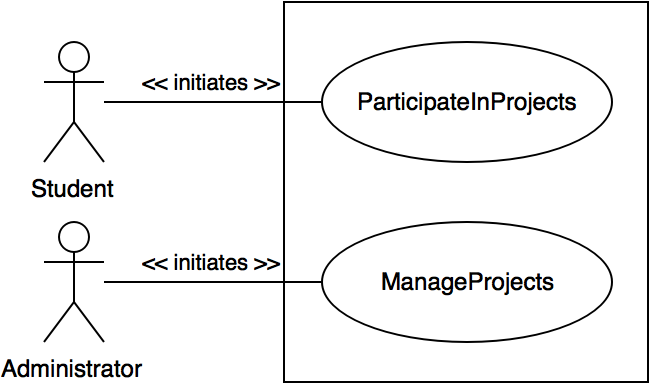
\includegraphics[scale=0.4]{imgs/high-level-use-case-diagram.png}
	\caption{High-level Use Case Diagram}
\end{figure}

\begin{table}[H]
\caption{High-Level Use Case Descriptions}
\renewcommand{\arraystretch}{1.5}
\everyrow{\hline}
\begin{tabu} to \textwidth {>{}l >{\bf}l X}
UC-01 & ManageProjectParticipation & description blah blah \\
UC-02 & ManageProjects & blah \\
\end{tabu}
\end{table}

\begin{figure}[H]
	\centering{}
	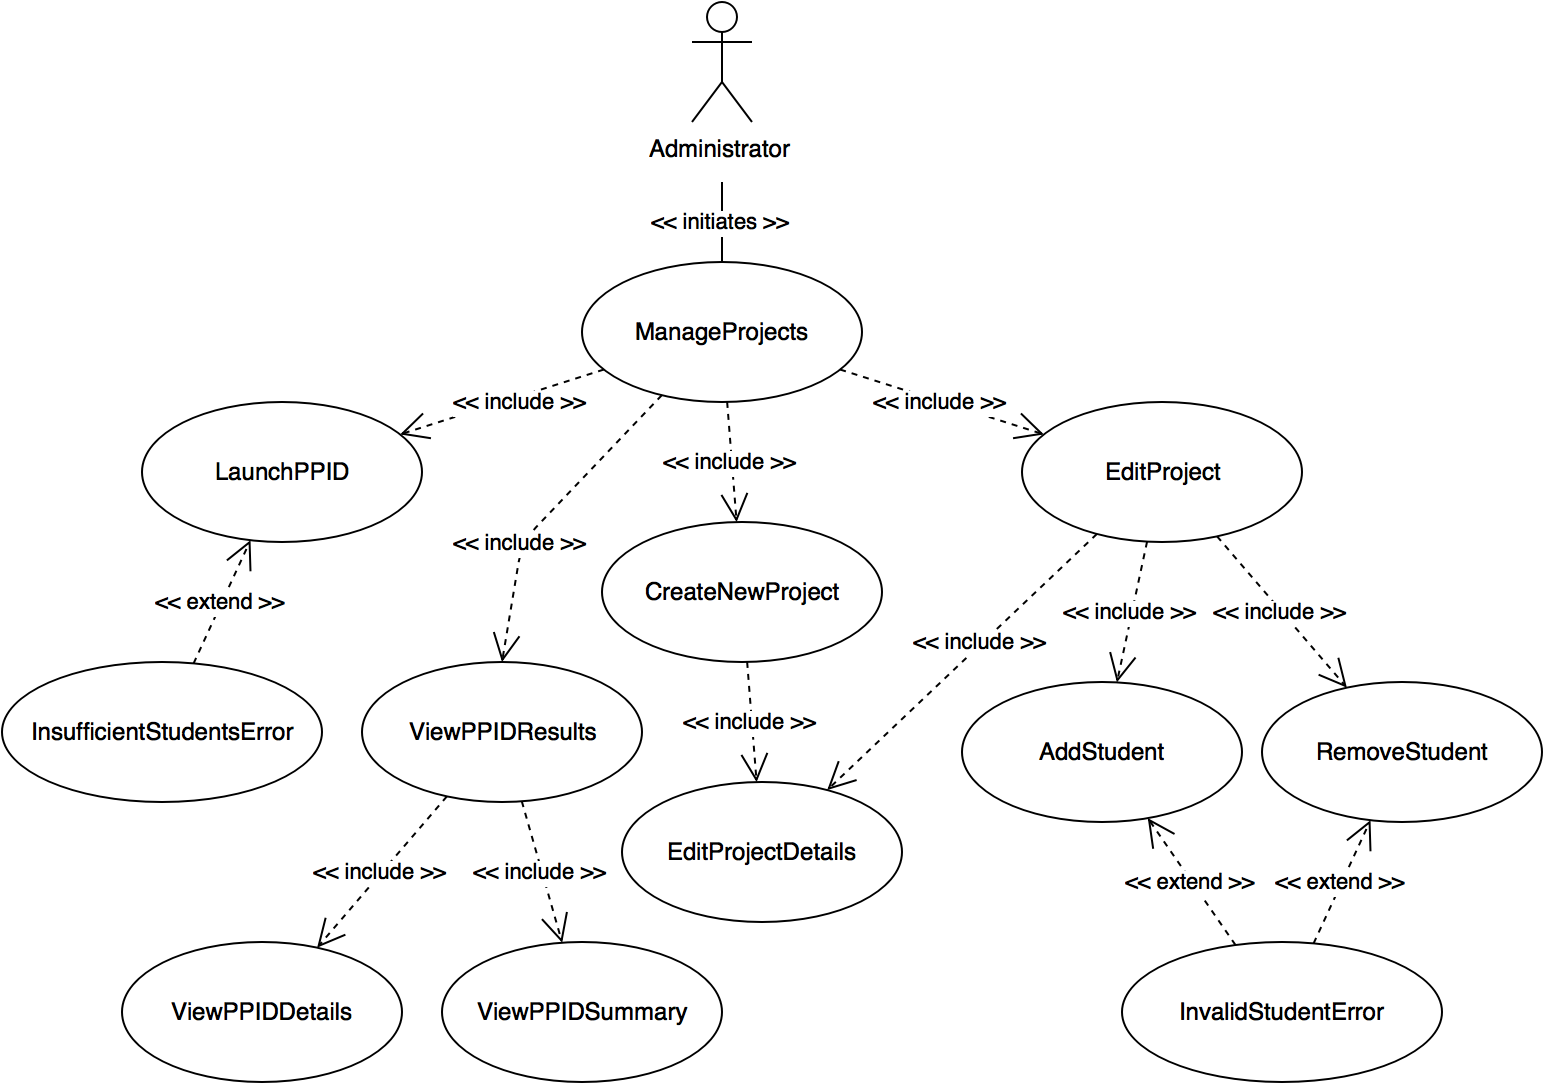
\includegraphics[scale=0.23]{imgs/detailed-administrator-use-case-diagram.png}
	\caption{Detailed Administrator Use Case Diagram}
\end{figure}

\begin{figure}[H]
	\centering{}
	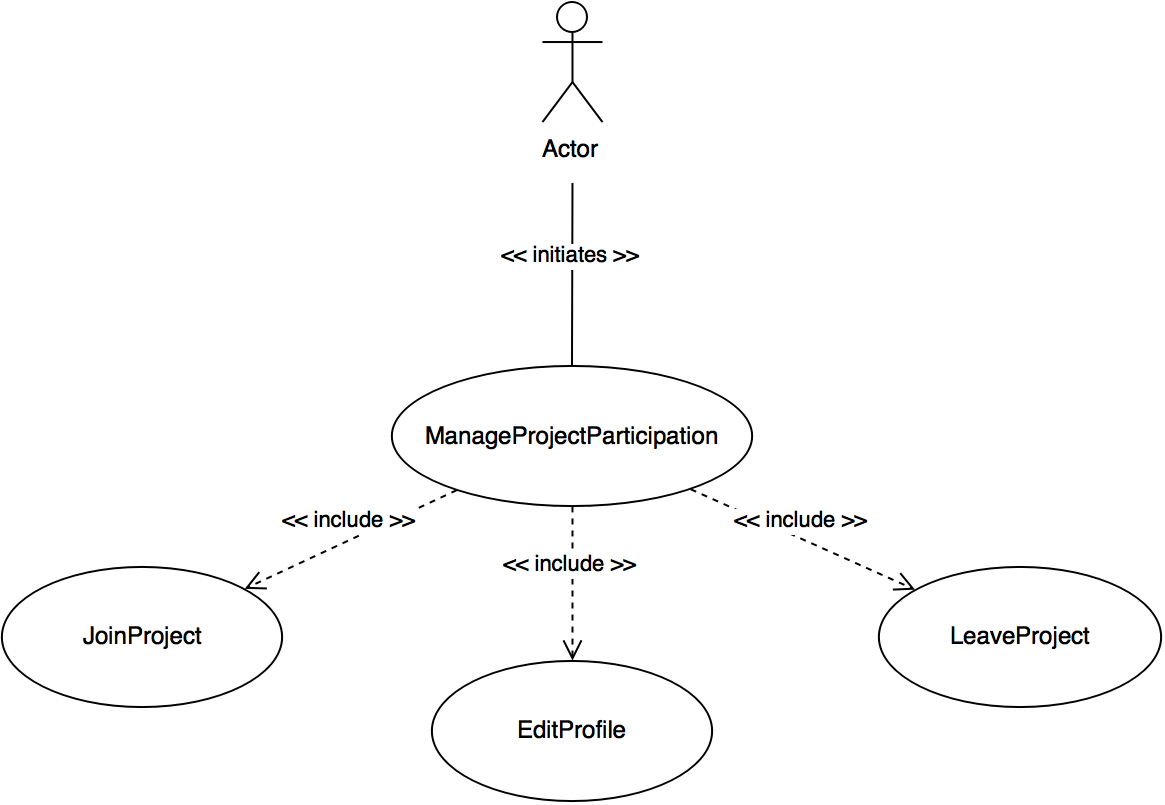
\includegraphics[scale=0.25]{imgs/detailed-student-use-case-diagram.png}
	\caption{Detailed Student Use Case Diagram}
\end{figure}

\begin{table}[H]
\caption{Detailed Use Case Descriptions}
\renewcommand{\arraystretch}{1.5}
\everyrow{\hline}
\begin{tabu} to \textwidth {>{}l >{\bf}l X}
UC-03 & ViewPPIDDetails & stuff\\
UC-04 & CreateNewProject & The Administrator creates a new instance of a project.\\
UC-05 & LaunchPPID & The Administrator applies the PPID Algorithm to a specified project.\\
UC-06 & ViewPPIDSummary & stuff\\
UC-07 & EditProject & The Administrator modifies the parameters of a specified project.\\
UC-08 & AddStudent & The Administrator adds a Student to the current project.\\
UC-09 & RemoveStudent & The Administrator removes a Student from the current project.\\
UC-10 & FileError & stuff\\
UC-11 & FileOpenError & stuff\\
UC-12 & FileInputError & stuff\\
UC-13 & FileOutputError & stuff\\
UC-14 & FileFormatError & stuff\\
UC-15 & InvalidInputError & stuff\\
UC-16 & NoStudentSelectedError & stuff\\
UC-17 & InsufficientStudentsError & stuff\\
\end{tabu}
\end{table}

\begin{center}
\renewcommand{\arraystretch}{1.5}
\everyrow{\hline}
\begin{tabu} to \textwidth {>{\it}l X}
\toprule
Use Case Identifier & UC-01 \\
Name & {\bf ManageProjectParticipation} \\
Participating Actors & Student \\
Flow of Events & blah \\
Entry Conditions & \textbullet \hspace{2 mm}blah \\
Exit Conditions & \textbullet \hspace{2 mm}blah \\
Quality Requirements & \textbullet \hspace{2 mm}blah \\
Traceability & \textbullet \hspace{2 mm}blah \\
\toprule
\end{tabu}
\end{center}

\begin{center}
\renewcommand{\arraystretch}{1.5}
\everyrow{\hline}
\begin{tabu} to \textwidth {>{\it}l X}
\toprule
Use Case Identifier & UC-02 \\
Name & {\bf ManageProjects} \\
Participating Actors & Administrator \\
Flow of Events & 1. The Administrator starts up the Administration process.
2.\\
Entry Conditions & \textbullet \hspace{2 mm}blah \\
Exit Conditions & \textbullet \hspace{2 mm}blah \\
Quality Requirements & \textbullet \hspace{2 mm}blah \\
Traceability & \textbullet \hspace{2 mm}blah \\
\toprule
\end{tabu}
\end{center}

\begin{center}
\renewcommand{\arraystretch}{1.5}
\everyrow{\hline}
\begin{tabu} to \textwidth {>{\it}l X}
\toprule
Use Case Identifier & UC-03 \\
Name & {\bf ViewPPIDDetails} \\
Participating Actors & Administrator \\
Flow of Events & stuff \\
Entry Conditions & \textbullet \hspace{2 mm}blah \\
Exit Conditions & \textbullet \hspace{2 mm}blah \\
Quality Requirements & \textbullet \hspace{2 mm}blah \\
Traceability & \textbullet \hspace{2 mm}F-09 \\
\toprule
\end{tabu}
\end{center}

\begin{center}
\renewcommand{\arraystretch}{1.5}
\everyrow{\hline}
\begin{tabu} to \textwidth {>{\it}l X}
\toprule
Use Case Identifier & UC-04 \\
Name & {\bf CreateNewProject} \\
Participating Actors & Administrator \\
Flow of Events & stuff \\
Entry Conditions & \textbullet \hspace{2 mm}blah \\
Exit Conditions & \textbullet \hspace{2 mm}blah \\
Quality Requirements & \textbullet \hspace{2 mm}blah \\
Traceability & \textbullet \hspace{2 mm}F-05 \\
\toprule
\end{tabu}
\end{center}

\begin{center}
\renewcommand{\arraystretch}{1.5}
\everyrow{\hline}
\begin{tabu} to \textwidth {>{\it}l X}
\toprule
Use Case Identifier & UC-05 \\
Name & {\bf LaunchPPID} \\
Participating Actors & Administrator \\
Flow of Events & stuff\\
Entry Conditions & \textbullet \hspace{2 mm}blah \\
Exit Conditions & \textbullet \hspace{2 mm}blah \\
Quality Requirements & \textbullet \hspace{2 mm}blah \\
Traceability & \textbullet \hspace{2 mm}F-07 \\
\toprule
\end{tabu}
\end{center}

\begin{center}
\renewcommand{\arraystretch}{1.5}
\everyrow{\hline}
\begin{tabu} to \textwidth {>{\it}l X}
\toprule
Use Case Identifier & UC-06 \\
Name & {\bf ViewPPIDSummary} \\
Participating Actors & Administrator \\
Flow of Events & stuff\\
Entry Conditions & \textbullet \hspace{2 mm}blah \\
Exit Conditions & \textbullet \hspace{2 mm}blah \\
Quality Requirements & \textbullet \hspace{2 mm}blah \\
Traceability & \textbullet \hspace{2 mm}F-08 \\
\toprule
\end{tabu}
\end{center}

\begin{center}
\renewcommand{\arraystretch}{1.5}
\everyrow{\hline}
\begin{tabu} to \textwidth {>{\it}l X}
\toprule
Use Case Identifier & UC-07 \\
Name & {\bf EditProject} \\
Participating Actors & Administrator \\
Flow of Events & stuff\\
Entry Conditions & \textbullet \hspace{2 mm}blah \\
Exit Conditions & \textbullet \hspace{2 mm}blah \\
Quality Requirements & \textbullet \hspace{2 mm}blah \\
Traceability & \textbullet \hspace{2 mm}F-06 \\
\toprule
\end{tabu}
\end{center}

\begin{center}
\renewcommand{\arraystretch}{1.5}
\everyrow{\hline}
\begin{tabu} to \textwidth {>{\it}l X}
\toprule
Use Case Identifier & UC-08 \\
Name & {\bf AddStudent} \\
Participating Actors & Administrator \\
Flow of Events & stuff\\
Entry Conditions & \textbullet \hspace{2 mm}blah \\
Exit Conditions & \textbullet \hspace{2 mm}blah \\
Quality Requirements & \textbullet \hspace{2 mm}blah \\
Traceability & \textbullet \hspace{2 mm}F-06-02 \\
\toprule
\end{tabu}
\end{center}

\begin{center}
\renewcommand{\arraystretch}{1.5}
\everyrow{\hline}
\begin{tabu} to \textwidth {>{\it}l X}
\toprule
Use Case Identifier & UC-09 \\
Name & {\bf RemoveStudent} \\
Participating Actors & Administrator \\
Flow of Events & stuff\\
Entry Conditions & \textbullet \hspace{2 mm}blah \\
Exit Conditions & \textbullet \hspace{2 mm}blah \\
Quality Requirements & \textbullet \hspace{2 mm}blah \\
Traceability & \textbullet \hspace{2 mm}F-06-03 \\
\toprule
\end{tabu}
\end{center}

\begin{center}
\renewcommand{\arraystretch}{1.5}
\everyrow{\hline}
\begin{tabu} to \textwidth {>{\it}l X}
\toprule
Use Case Identifier & UC-10 \\
Name & {\bf FileError} \\
Participating Actors & Administrator \\
Flow of Events & stuff\\
Entry Conditions & \textbullet \hspace{2 mm}blah \\
Exit Conditions & \textbullet \hspace{2 mm}blah \\
Quality Requirements & \textbullet \hspace{2 mm}blah \\
Traceability & \textbullet \hspace{2 mm}NF-02 \\
\toprule
\end{tabu}
\end{center}

\begin{center}
\renewcommand{\arraystretch}{1.5}
\everyrow{\hline}
\begin{tabu} to \textwidth {>{\it}l X}
\toprule
Use Case Identifier & UC-11 \\
Name & {\bf FileOpenError} \\
Participating Actors & Administrator \\
Flow of Events & stuff\\
Entry Conditions & \textbullet \hspace{2 mm}blah \\
Exit Conditions & \textbullet \hspace{2 mm}blah \\
Quality Requirements & \textbullet \hspace{2 mm}blah \\
Traceability & \textbullet \hspace{2 mm}NF-02 \\
\toprule
\end{tabu}
\end{center}

\begin{center}
\renewcommand{\arraystretch}{1.5}
\everyrow{\hline}
\begin{tabu} to \textwidth {>{\it}l X}
\toprule
Use Case Identifier & UC-12 \\
Name & {\bf FileInputError} \\
Participating Actors & Administrator \\
Flow of Events & stuff\\
Entry Conditions & \textbullet \hspace{2 mm}blah \\
Exit Conditions & \textbullet \hspace{2 mm}blah \\
Quality Requirements & \textbullet \hspace{2 mm}blah \\
Traceability & \textbullet \hspace{2 mm}NF-02 \\
\toprule
\end{tabu}
\end{center}

\begin{center}
\renewcommand{\arraystretch}{1.5}
\everyrow{\hline}
\begin{tabu} to \textwidth {>{\it}l X}
\toprule
Use Case Identifier & UC-13 \\
Name & {\bf FileOutputError} \\
Participating Actors & Administrator \\
Flow of Events & stuff\\
Entry Conditions & \textbullet \hspace{2 mm}blah \\
Exit Conditions & \textbullet \hspace{2 mm}blah \\
Quality Requirements & \textbullet \hspace{2 mm}blah \\
Traceability & \textbullet \hspace{2 mm}NF-02 \\
\toprule
\end{tabu}
\end{center}

\begin{center}
\renewcommand{\arraystretch}{1.5}
\everyrow{\hline}
\begin{tabu} to \textwidth {>{\it}l X}
\toprule
Use Case Identifier & UC-14 \\
Name & {\bf FileFormatError} \\
Participating Actors & Administrator \\
Flow of Events & stuff\\
Entry Conditions & \textbullet \hspace{2 mm}blah \\
Exit Conditions & \textbullet \hspace{2 mm}blah \\
Quality Requirements & \textbullet \hspace{2 mm}blah \\
Traceability & \textbullet \hspace{2 mm}NF-02 \\
\toprule
\end{tabu}
\end{center}

\begin{center}
\renewcommand{\arraystretch}{1.5}
\everyrow{\hline}
\begin{tabu} to \textwidth {>{\it}l X}
\toprule
Use Case Identifier & UC-15 \\
Name & {\bf InvalidFormatError} \\
Participating Actors & Administrator \\
Flow of Events & stuff\\
Entry Conditions & \textbullet \hspace{2 mm}blah \\
Exit Conditions & \textbullet \hspace{2 mm}blah \\
Quality Requirements & \textbullet \hspace{2 mm}blah \\
Traceability & \textbullet \hspace{2 mm}NF-02 \\
\toprule
\end{tabu}
\end{center}

\begin{center}
\renewcommand{\arraystretch}{1.5}
\everyrow{\hline}
\begin{tabu} to \textwidth {>{\it}l X}
\toprule
Use Case Identifier & UC-16 \\
Name & {\bf NoStudentSelectedError} \\
Participating Actors & Administrator \\
Flow of Events & stuff\\
Entry Conditions & \textbullet \hspace{2 mm}blah \\
Exit Conditions & \textbullet \hspace{2 mm}blah \\
Quality Requirements & \textbullet \hspace{2 mm}blah \\
Traceability & \textbullet \hspace{2 mm}NF-02 \\
\toprule
\end{tabu}
\end{center}

\begin{center}
\renewcommand{\arraystretch}{1.5}
\everyrow{\hline}
\begin{tabu} to \textwidth {>{\it}l X}
\toprule
Use Case Identifier & UC-17 \\
Name & {\bf InsufficientStudentsError} \\
Participating Actors & Administrator \\
Flow of Events & stuff\\
Entry Conditions & \textbullet \hspace{2 mm}blah \\
Exit Conditions & \textbullet \hspace{2 mm}blah \\
Quality Requirements & \textbullet \hspace{2 mm}blah \\
Traceability & \textbullet \hspace{2 mm}NF-02 \\
\toprule
\end{tabu}
\end{center}

\subsubsection{Object Model}


\subsubsection{Dynamic Model}


\end{document}
